% Name: Phase portrait
% Description: Trajectories of the pendulum, theta'' = -sin theta, in the phase plane: closed orbits around the center, the separatrix through the two saddles, and rotations above and below.
% Tags: phase portrait, phase plane, pendulum, dynamical systems

\usepackage{pgfplots}
\usetikzlibrary{decorations.markings}
\pgfplotsset{compat=1.18}

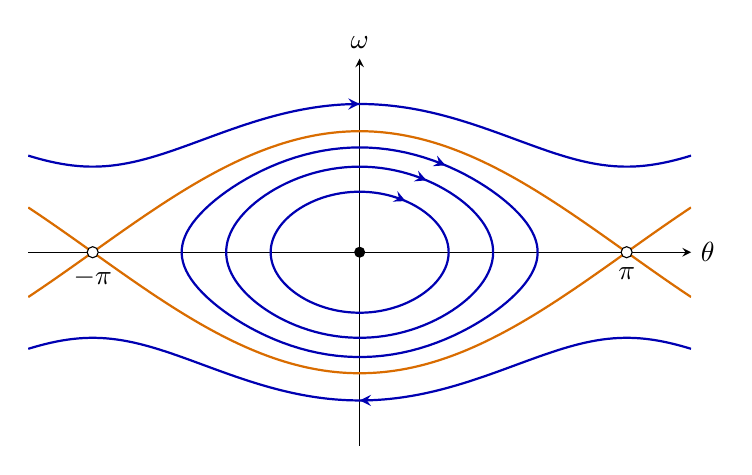
\begin{tikzpicture}[flow/.style={postaction={decorate}, decoration={markings, mark=at position #1 with {\arrow{stealth}}}}]
  \begin{axis}[
    width=10cm, height=6.5cm, axis lines=middle, xlabel=$\theta$, ylabel=$\omega$,
    xmin=-3.9, xmax=3.9, ymin=-3.2, ymax=3.2, xtick={-3.1416,3.1416}, xticklabels={$-\pi$, $\pi$},
    ytick=\empty, every axis plot/.append style={thick, blue!70!black, samples=120},
    xlabel style={anchor=west}, ylabel style={anchor=south},
  ]
    % Each orbit keeps the energy E = omega^2/2 - cos(theta); a closed orbit reaches theta_max = acos(-E).
    \pgfplotsinvokeforeach{-0.5, 0, 0.5}{
      \addplot[flow=0.1, domain=0:360, variable=\s]
        ({acos(-#1)*pi/180*sin(s)}, {sign(cos(s))*sqrt(max(0, 2*(#1 + cos(acos(-#1)*sin(s)))))});
    }
    % The separatrix (E = 1) is omega = 2 cos(theta/2); the rotations have E = 2.
    \addplot[orange!85!black, domain=-3.9:3.9] {2*abs(cos(deg(x)/2))};
    \addplot[orange!85!black, domain=-3.9:3.9] {-2*abs(cos(deg(x)/2))};
    \addplot[flow=0.5, domain=-3.9:3.9] {sqrt(2*(2 + cos(deg(x))))};
    \addplot[flow=0.5, domain=3.9:-3.9] {-sqrt(2*(2 + cos(deg(x))))};
    \fill[black] (axis cs:0,0) circle (2pt);
    \filldraw[fill=white, draw=black] (axis cs:-3.1416,0) circle (2pt) (axis cs:3.1416,0) circle (2pt);
  \end{axis}
\end{tikzpicture}
